\section{Implementation}
Here we describe our implementation of a Naive Bayes spam classifier. Further documentation is available with the package.

The project has been written in Python. It requires two external modules, \verb!bs4! (\verb!BeautifulSoup!) to parse a text and \verb!Ply! to perform the lexical analysis of a text.

\subsection{Structure}
The package is composed as follows:
\begin{description}[noitemsep]
  \item[spam\_bayes] the module contianing the \verb!__main__! class;
  \item[naive\_bayes] the module defining the Bayesian network;
  \item[config] contains some general configurations, manages the settings defined by the user;
  \item[trainer] contains the trainer;
  \item[classifier] applies the Bayesian logic to classify a mail;
  \item[lexer] implementing the lexical analyzer to compute the statistics;
  \item[utils] with some methods used in more classes.
  \item[gen\_stat] defines the objects to describe the statistics for words and features of the global network;
  \item[test\_stat] defines the objects to describe the statistics for words and features of a single mail of unknown status.
\end{description}

Image \ref{fig:uml} shows the interconnection between the classes.
\begin{figure}[h]
  \begin{center}
    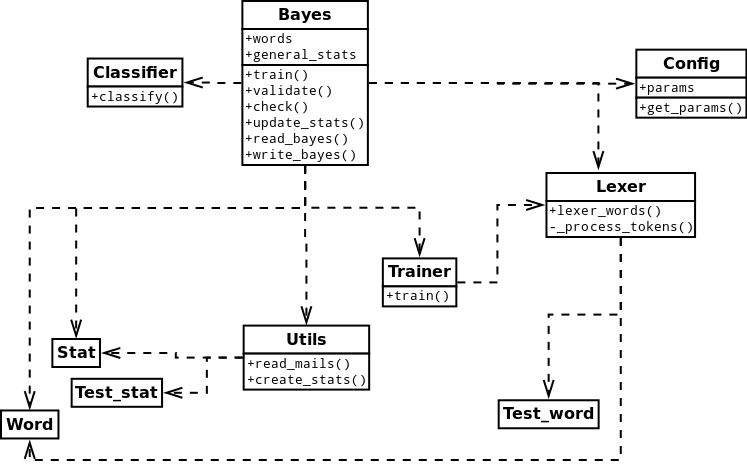
\includegraphics[width=0.6\textwidth]{img/uml.png}
    \caption{UML diagram of the classes.}
    \label{fig:uml}
  \end{center}
\end{figure}

The file \verb!spam_bayes.conf! allows the user to configure the parameters.

\subsubsection{Notes on implementation}
In section \ref{computeprob} we have discussed how to compute the probability of being spam and ham, and we have discarded the total probability of each word, since it's only a normalizer, equal for both the terms. We can further simplify the calculation, assuming to not know the a priori probability for a mail to be spam or ham, and so considering it $0.5$. This is true when the classification begins, and the bag of words is still empty, or when the number of spam and ham mails are almost equal. However, this works also when there is a disproportion between the numbers of spam and ham mails. Thus, being this probability equal for both terms, it can be discarded.

We need also to be careful when computing the total probability, since if the probability of being spam or ham associated to a word is $0$ (e.g. no spam/ham mails contain the word), the total probability will be $0$ regardless of all the other probabilities. To avoid this, we add a smoothing value to both the numerator and denominator in $P_{spam|word}$ and $P_{ham|word}$. Thus, the formula for spam becomes $$P_{word|spam} = \frac{\mbox{\# occurrences of word in spam mails} + k}{\mbox{\# total occurrences of the word} + |C|\times k},$$ where $|C|$ is the number of possible classes, in our case 2, spam and ham, and $k > 0$ is the smooth value. If $k=1$ it is called Laplace smoothing.

Furthermore, other calculation can be avoided. Words like articles or conjunctions are very common in every meaningful text, so we expect them to appear many times in both spam and ham mails. We can extend this observation, considering that every word which has a probability of being spam close to $0.5$ will also have a very similar probability of being ham, since their sum has to be $1$. Thus, also these words bring very little contribution to the spamminess of a mail, and can therefore be ignored. We provide a customizable threshold to allow the user to set the preferred deviation from the half, for the word to be counted into the probability.
